\documentclass{exam}
\usepackage{graphicx}
\usepackage{xcolor}
\usepackage{framed}
\usepackage{amssymb}
\usepackage[utf8]{inputenc}
\usepackage{textcomp}

% Format Header and footer
\pagestyle{headandfoot}
\header{\footnotesize Klass:\\Namn:}{\Large\textbf{Fysiologi II - Bedömningsanvisningar}\\\medskip\small Nervsystemet, rörelseapparaten och endokrina organsystemet}{\footnotesize BIOBIO02 - 2025\\Viktor Arohlén}
\headrule
\footrule
\setlength{\columnsep}{0.25cm}
\footer{}{Sida \thepage}{}

\newenvironment{answer}
  {\begin{framed}\color{blue}\textbf{Bedömning:} }
  {\end{framed}}

\begin{document}
\section*{Instruktioner}
Provet består av två delar \\
    - Grundläggande frågor, svara kortfattat (\textit{14 poäng})\\
    - Fördjupande frågor, svara mer omfattande (\textit{10 poäng} + 2 bonuspoäng)

\subsection*{Poäng}
Antalet poäng är markerat för varje fråga. Totalt \textbf{12 frågor} och \textbf{24 poäng}.\\ \textit{För godkänt resultat krävs 10 poäng.}

\vspace{5mm} %5mm vertical space
\begin{center}
\fbox{\fbox{\parbox{6in}{\centering
\textbf{Grundläggande frågor}: svara kortfattat (\textbf{14 poäng})
}}}
\end{center}
\begin{questions}

\question I vilken ordning sker de olika stegen i en aktionspotential i en nervcell? (\textbf{2 poäng})

\begin{itemize}
  \item Repolarisation av membranet
  \item Spänningsstyrda kaliumkanaler öppnas – kalium strömmar ut
  \item En retning når tröskelvärdet
  \item Spänningsstyrda natriumkanaler öppnas – natrium strömmar in
  \item Depolarisation av membranet
  \item Hyperpolarisation (refraktärperiod)
  \item Vilopotential upprätthålls av natrium-kaliumpumpen
\end{itemize}

\begin{answer}
\textbf{Korrekt ordning:}
\begin{enumerate}
  \item Vilopotential upprätthålls av natrium-kaliumpumpen
  \item En retning når tröskelvärdet
  \item Spänningsstyrda natriumkanaler öppnas – natrium strömmar in
  \item Depolarisation av membranet
  \item Spänningsstyrda kaliumkanaler öppnas – kalium strömmar ut
  \item Repolarisation av membranet
  \item Hyperpolarisation (refraktärperiod)
\end{enumerate}

\textbf{Poängbedömning:}
\begin{itemize}
  \item 2 poäng: Korrekt ordning på alla steg
  \item 1 poäng: Minst 5 steg i korrekt ordning
  \item 0 poäng: Färre än 5 steg i korrekt ordning
\end{itemize}
\end{answer}
\vspace{5mm} %5mm vertical space

\question Ge exempel på en \textbf{äkta led} och en \textbf{oäkta led} och vad de har för likheter och skillnader. (\textbf{2 poäng})
\vspace{10mm}

\begin{answer}
\textbf{Korrekt svar:}

\textbf{Äkta led (synovialled):} T.ex. knäled, armbågsled, höftled, axelled.
\begin{itemize}
  \item Har ledkapsel med ledvätska
  \item Ledhuvud och ledpanna täckta av ledbrosk
  \item Möjliggör större rörlighet
\end{itemize}

\textbf{Oäkta led:} T.ex. fogarna mellan ryggkotor, bäckenfogen, skallens fogar.
\begin{itemize}
  \item Saknar ledkapsel och ledvätska
  \item Förbinds av bindväv, brosk eller ben
  \item Mer begränsad rörlighet
\end{itemize}

\textbf{Likheter:}
\begin{itemize}
  \item Båda förbinder ben med varandra
  \item Båda möjliggör viss rörlighet (om än i olika grad)
\end{itemize}

\textbf{Skillnader:}
\begin{itemize}
  \item Äkta leder har ledkapsel och ledvätska, oäkta leder saknar detta
  \item Äkta leder har större rörlighet än oäkta leder
  \item Äkta leder har ledbrosk, oäkta leder har andra typer av vävnad mellan benen
\end{itemize}

\textbf{Poängbedömning:}
\begin{itemize}
  \item 2 poäng: Korrekt exempel på både äkta och oäkta led, samt relevanta likheter och skillnader
  \item 1 poäng: Korrekt exempel på antingen äkta eller oäkta led, samt några likheter eller skillnader
  \item 0 poäng: Felaktiga exempel eller avsaknad av likheter och skillnader
\end{itemize}
\end{answer}
\vspace{5mm}
\question Vad av följande \textbf{stämmer} om nervsystemet? (\textbf{2 poäng})
\begin{checkboxes}
    \choice Parasympatiska nervsystemet aktiveras vid fysisk ansträngning
    \choice Sympatiska nervsystemet sänker hjärtfrekvensen
    \choice \textcolor{blue}{\checkmark} Somatiska nervsystemet styr viljestyrda rörelser
    \choice Autonoma nervsystemet kontrollerar skelettmuskulatur
    \choice \textcolor{blue}{\checkmark} Sensoriska nerver skickar signaler till hjärnan
    \choice Det perifera nervsystemet består av hjärna och ryggmärg
    \choice \textcolor{blue}{\checkmark} Det autonoma nervsystemet styr hjärtat
    \choice \textcolor{blue}{\checkmark} Motoriska nerver leder signaler från hjärnan till muskler
\end{checkboxes}

\begin{answer}
\textbf{Korrekta påståenden:}
\begin{itemize}
  \item Somatiska nervsystemet styr viljestyrda rörelser
  \item Sensoriska nerver skickar signaler till hjärnan
  \item Det autonoma nervsystemet styr hjärtat
  \item Motoriska nerver leder signaler från hjärnan till muskler
\end{itemize}

\textbf{Felaktiga påståenden:}
\begin{itemize}
  \item Parasympatiska nervsystemet aktiveras vid fysisk ansträngning (Fel: Det sympatiska nervsystemet aktiveras vid fysisk ansträngning, "fight or flight")
  \item Sympatiska nervsystemet sänker hjärtfrekvensen (Fel: Det sympatiska nervsystemet höjer hjärtfrekvensen)
  \item Autonoma nervsystemet kontrollerar skelettmuskulatur (Fel: Det somatiska nervsystemet kontrollerar skelettmuskulatur)
  \item Det perifera nervsystemet består av hjärna och ryggmärg (Fel: Det centrala nervsystemet består av hjärna och ryggmärg)
\end{itemize}

\textbf{Poängbedömning:}
\begin{itemize}
  \item 2 poäng: Alla fyra rätta alternativ markerade och inga felaktiga
  \item 1,5 poäng: Tre rätta alternativ markerade och inga felaktiga
  \item 1 poäng: Två rätta alternativ markerade och inga felaktiga, eller tre-fyra rätta med ett felaktigt
  \item 0,5 poäng: Ett rätt alternativ markerat och inga felaktiga, eller två rätta med ett felaktigt
  \item 0 poäng: Inget rätt alternativ markerat eller fler felaktiga än rätta
\end{itemize}
\end{answer}

\break
\question Nämn en av de endorkina körtlarna och ge ett exempel på vilket hormon som produceras och vad det påverkar. (\textbf{2 poäng})
\begin{figure}[h]
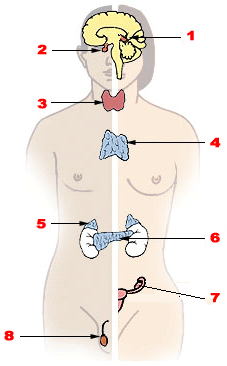
\includegraphics[width=0.2\textwidth]{endokrina.png}
\end{figure}
\vspace{5mm}

\begin{answer}
\textbf{Korrekt svar:}

Exempel på endokrina körtlar och deras hormoner:
\begin{itemize}
  \item \textbf{Hypofysen:} Tillväxthormon (GH) - stimulerar tillväxt och celldelning, ADH - reglerar vattenbalans, Oxytocin - stimulerar livmodersammandragningar vid förlossning
  \item \textbf{Sköldkörteln:} Tyroxin (T4) och trijodtyronin (T3) - reglerar ämnesomsättningen
  \item \textbf{Binjurarna:} Adrenalin - höjer blodtryck och puls vid stress, Kortisol - reglerar metabolism och immunförsvar
  \item \textbf{Bukspottkörteln:} Insulin - sänker blodsockret, Glukagon - höjer blodsockret
  \item \textbf{Könskörtlarna (äggstockar/testiklar):} Östrogen/testosteron - påverkar könsutveckling och reproduktion
  \item \textbf{Bisköldkörtlarna:} Parathormon - reglerar kalciumbalansen i blodet
  \item \textbf{Tallkottkörteln (epifysen):} Melatonin - reglerar dygnsrytm och sömn
\end{itemize}

\textbf{Poängbedömning:}
\begin{itemize}
  \item 2 poäng: Korrekt identifiering av en endokrin körtel, samt korrekt beskrivning av ett hormon den producerar och dess funktion
  \item 1 poäng: Korrekt identifiering av en endokrin körtel, men ofullständig eller delvis felaktig beskrivning av hormon eller funktion
  \item 0 poäng: Felaktig identifiering av endokrin körtel eller helt felaktig beskrivning av hormon och funktion
\end{itemize}
\end{answer}
\vspace{5mm}

\question Varför har vi olika typer av \textbf{muskelvävnad} i kroppen? (\textbf{2 poäng})
\vspace{10mm}

\begin{answer}
\textbf{Korrekt svar:}

Vi har tre huvudtyper av muskelvävnad i kroppen, var och en med specifika egenskaper och funktioner:

\begin{itemize}
  \item \textbf{Skelettmuskulatur (tvärstrimmig, viljestyrd):}
  \begin{itemize}
    \item Fäster vid skelettet och möjliggör rörelse
    \item Viljestyrd (kontrolleras medvetet)
    \item Snabb kontraktion men tröttas relativt snabbt
    \item Exempel: biceps, quadriceps
  \end{itemize}
  
  \item \textbf{Hjärtmuskulatur (tvärstrimmig, icke-viljestyrd):}
  \begin{itemize}
    \item Finns endast i hjärtat
    \item Icke-viljestyrd (autonom)
    \item Rytmisk, uthållig kontraktion utan trötthet
    \item Specialiserad för kontinuerligt arbete
  \end{itemize}
  
  \item \textbf{Glatt muskulatur (icke-tvärstrimmig, icke-viljestyrd):}
  \begin{itemize}
    \item Finns i inre organ, blodkärl, tarm, etc.
    \item Icke-viljestyrd (autonom)
    \item Långsam, uthållig kontraktion
    \item Kontrollerar funktioner som peristaltik, blodkärlsdiameter, etc.
  \end{itemize}
\end{itemize}

De olika typerna av muskelvävnad behövs för att kroppen ska kunna utföra olika typer av rörelser och funktioner med varierande krav på hastighet, uthållighet, styrka och kontroll.

\textbf{Poängbedömning:}
\begin{itemize}
  \item 2 poäng: Beskrivning av minst två typer av muskelvävnad med korrekta egenskaper och förklaring till varför de olika typerna behövs
  \item 1 poäng: Beskrivning av minst en typ av muskelvävnad med korrekta egenskaper eller ofullständig beskrivning av flera typer
  \item 0 poäng: Felaktig eller mycket ofullständig beskrivning
\end{itemize}
\end{answer}
\vspace{5mm}

\question Ge exempel på två olika \textbf{signalsubstanser (neurotransmittorer)} och deras funktion. (\textbf{2 poäng})
\vspace{5mm}

\begin{answer}
\textbf{Korrekt svar:}

Exempel på signalsubstanser och deras funktioner:
\begin{itemize}
  \item \textbf{Acetylkolin:} 
  \begin{itemize}
    \item Funktion vid muskelkontraktion (neuromuskulära synapser)
    \item Viktig för inlärning och minne i hjärnan
    \item Aktiverar det parasympatiska nervsystemet ("rest and digest")
  \end{itemize}
  
  \item \textbf{Dopamin:}
  \begin{itemize}
    \item Involverad i belöningssystemet och motivation
    \item Reglerar motorisk kontroll
    \item Påverkar humör och välbefinnande
  \end{itemize}
  
  \item \textbf{Serotonin:}
  \begin{itemize}
    \item Reglerar humör, sömn och aptit
    \item Påverkar social beteende och välbefinnande
    \item Involverad i reglering av kroppstemperatur
  \end{itemize}
  
  \item \textbf{Noradrenalin:}
  \begin{itemize}
    \item Aktiverar det sympatiska nervsystemet ("fight or flight")
    \item Ökar vakenhet och uppmärksamhet
    \item Påverkar blodtryck och hjärtfrekvens
  \end{itemize}
  
  \item \textbf{GABA (gamma-aminosmörsyra):}
  \begin{itemize}
    \item Huvudsaklig hämmande signalsubstans i hjärnan
    \item Minskar nervaktivitet och har lugnande effekt
    \item Viktig för att balansera excitation och inhibition
  \end{itemize}
  
  \item \textbf{Glutamat:}
  \begin{itemize}
    \item Huvudsaklig excitatorisk signalsubstans i hjärnan
    \item Viktig för inlärning och minne
    \item Involverad i synaptisk plasticitet
  \end{itemize}
\end{itemize}

\textbf{Poängbedömning:}
\begin{itemize}
  \item 2 poäng: Korrekt beskrivning av två signalsubstanser och deras funktioner
  \item 1 poäng: Korrekt beskrivning av en signalsubstans och dess funktion, eller ofullständig beskrivning av två
  \item 0 poäng: Felaktig eller mycket ofullständig beskrivning
\end{itemize}
\end{answer}
\vspace{5mm}

\question Vad av följande \textbf{stämmer} om skelettet? (\textbf{2 poäng})
\begin{checkboxes}
    \choice \textcolor{blue}{\checkmark} Skelettet skyddar inre organ.
    \choice Alla ben i kroppen är ihåliga.
    \choice \textcolor{blue}{\checkmark} Skelettet lagrar mineraler som kalcium och fosfat.
    \choice \textcolor{blue}{\checkmark} Röd benmärg bildar blodkroppar.
    \choice Skelettet består bara av död vävnad.
    \choice \textcolor{blue}{\checkmark} Leder förbinder olika ben i skelettet.
    \choice \textcolor{blue}{\checkmark} Skelettet är viktigt för kroppens rörelse.
    \choice Skelettet producerar hormoner som insulin.
\end{checkboxes}

\begin{answer}
\textbf{Korrekta påståenden:}
\begin{itemize}
  \item Skelettet skyddar inre organ.
  \item Skelettet lagrar mineraler som kalcium och fosfat.
  \item Röd benmärg bildar blodkroppar.
  \item Leder förbinder olika ben i skelettet.
  \item Skelettet är viktigt för kroppens rörelse.
\end{itemize}

\textbf{Felaktiga påståenden:}
\begin{itemize}
  \item Alla ben i kroppen är ihåliga. (Fel: Vissa ben är kompakta, andra är ihåliga)
  \item Skelettet består bara av död vävnad. (Fel: Ben är levande vävnad med celler som ständigt ombildas)
  \item Skelettet producerar hormoner som insulin. (Fel: Insulin produceras i bukspottkörteln. Skelettet kan producera vissa hormoner som osteocalcin, men inte insulin)
\end{itemize}

\textbf{Poängbedömning:}
\begin{itemize}
  \item 2 poäng: Minst 4 rätta alternativ markerade och inga felaktiga
  \item 1,5 poäng: 3 rätta alternativ markerade och inga felaktiga
  \item 1 poäng: 2 rätta alternativ markerade och inga felaktiga, eller 3-4 rätta med ett felaktigt
  \item 0,5 poäng: 1 rätt alternativ markerat och inga felaktiga, eller 2 rätta med ett felaktigt
  \item 0 poäng: Inget rätt alternativ markerat eller fler felaktiga än rätta
\end{itemize}
\end{answer}
\break

\vspace{5mm} %5mm vertical space
\begin{center}
\fbox{\fbox{\parbox{6in}{\centering
\textbf{Fördjupande frågor}: svara mer utförligt (\textbf{10 poäng} + 2 bonuspoäng)
}}}
\end{center}

\question
Utifrån bilden beskriv hur en signal överförs mellan två nervceller. Använd relevanta begrepp. (\textbf{3 poäng})
\begin{figure}[h]
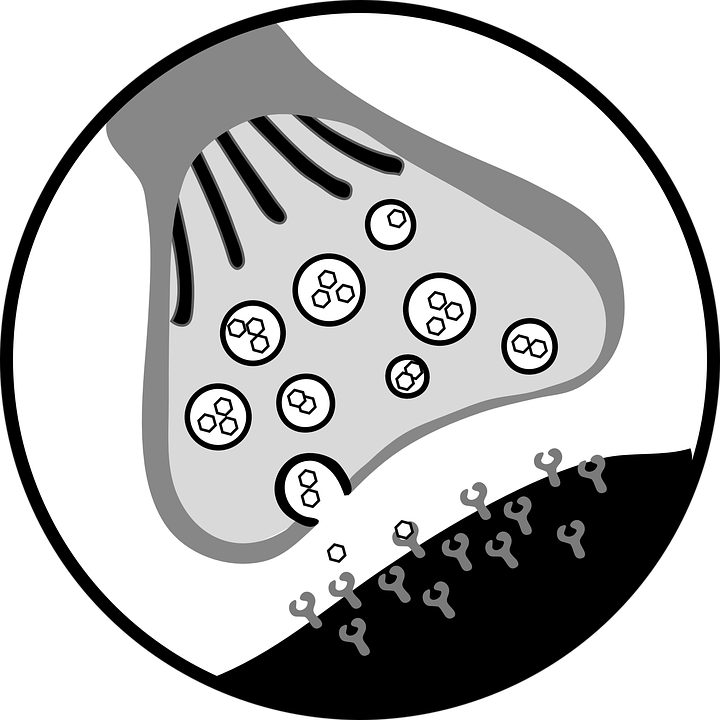
\includegraphics[width=0.4\textwidth]{synaps.png}
\end{figure}
\vspace{10mm}

\begin{answer}
\textbf{Korrekt svar:}

Signalöverföring mellan två nervceller (synaptisk transmission):

\begin{enumerate}
  \item \textbf{Aktionspotential:} En elektrisk signal (aktionspotential) färdas längs den presynaptiska neuronens axon.
  
  \item \textbf{Ankomst till synapsen:} När aktionspotentialen når axonterminalen (den presynaptiska terminalen) öppnas spänningskänsliga kalciumkanaler.
  
  \item \textbf{Kalciuminflöde:} Kalciumjoner (Ca$^{2+}$) strömmar in i den presynaptiska terminalen.
  
  \item \textbf{Frisättning av signalsubstanser:} Kalciuminflödet får vesiklar med signalsubstanser (neurotransmittorer) att smälta samman med cellmembranet genom exocytos.
  
  \item \textbf{Diffusion över synaptiska klyftan:} Signalsubstanserna frisätts i den synaptiska klyftan (spalten mellan cellerna) och diffunderar över till den postsynaptiska neuronen.
  
  \item \textbf{Bindning till receptorer:} Signalsubstanserna binder till specifika receptorer på den postsynaptiska neuronens membran.
  
  \item \textbf{Jonkanaler öppnas/stängs:} Beroende på typ av receptor och signalsubstans öppnas eller stängs jonkanaler i det postsynaptiska membranet.
  
  \item \textbf{Postsynaptisk potential:} Detta leder till antingen en excitatorisk postsynaptisk potential (EPSP, depolarisering) eller en inhibitorisk postsynaptisk potential (IPSP, hyperpolarisering).
  
  \item \textbf{Summering:} Om tillräckligt många excitatoriska signaler summeras och når tröskelvärdet, utlöses en ny aktionspotential i den postsynaptiska neuronen.
  
  \item \textbf{Avslutning av signalering:} Signalsubstanserna inaktiveras genom:
  \begin{itemize}
    \item Återupptag till den presynaptiska neuronen
    \item Enzymatisk nedbrytning i den synaptiska klyftan
    \item Diffusion bort från synapsen
  \end{itemize}
\end{enumerate}

\textbf{Poängbedömning:}
\begin{itemize}
  \item 3 poäng: Utförlig beskrivning av signalöverföringen med minst 7-8 av stegen ovan och korrekt användning av relevanta begrepp
  \item 2 poäng: God beskrivning av signalöverföringen med minst 5-6 av stegen ovan och viss användning av relevanta begrepp
  \item 1 poäng: Grundläggande beskrivning av signalöverföringen med minst 3-4 av stegen ovan
  \item 0 poäng: Felaktig eller mycket ofullständig beskrivning
\end{itemize}
\end{answer}
\vspace{5mm}

\question
Organismer har två olika system för kommunikation. Nervsystemet och det endokrina systemet. Vad är för- och nackdelarna med de olika systemen och varför är det viktigt att ha båda två? (\textbf{3 poäng})

\vspace{10mm}

\begin{answer}
\textbf{Korrekt svar:}

\textbf{Nervsystemet:}
\begin{itemize}
  \item \textbf{Fördelar:}
  \begin{itemize}
    \item Mycket snabb signalöverföring (millisekunder)
    \item Hög precision - signaler går till specifika målceller
    \item Möjliggör omedelbar respons på stimuli
    \item Kan kontrollera snabba och precisa rörelser
  \end{itemize}
  
  \item \textbf{Nackdelar:}
  \begin{itemize}
    \item Begränsad räckvidd - signaler går bara dit nerver når
    \item Kortvarig effekt - signaler avklingar snabbt
    \item Energikrävande
    \item Kräver direkta fysiska kopplingar (synapser) mellan celler
  \end{itemize}
\end{itemize}

\textbf{Endokrina systemet:}
\begin{itemize}
  \item \textbf{Fördelar:}
  \begin{itemize}
    \item Kan påverka hela kroppen samtidigt
    \item Långvarig effekt - hormoner kan verka under längre tid
    \item Kan reglera långsamma processer (t.ex. tillväxt, metabolism)
    \item Kräver inte direkta fysiska kopplingar mellan celler
  \end{itemize}
  
  \item \textbf{Nackdelar:}
  \begin{itemize}
    \item Långsam signalöverföring (sekunder till dagar)
    \item Mindre precision - hormoner transporteras via blodet till hela kroppen
    \item Inte lämpligt för snabba, precisa responser
  \end{itemize}
\end{itemize}

\textbf{Varför båda systemen behövs:}
\begin{itemize}
  \item Kompletterar varandra för att hantera olika typer av fysiologiska behov
  \item Nervsystemet hanterar snabba responser (t.ex. reflexer, rörelser)
  \item Endokrina systemet hanterar långsamma, omfattande processer (t.ex. tillväxt, metabolism, reproduktion)
  \item Många processer kräver samordning mellan båda systemen (t.ex. stressrespons)
  \item Tillsammans ger de organismen förmåga att anpassa sig till både snabba förändringar och långsiktiga behov
  \item Vissa funktioner kräver både nervös och hormonell reglering för optimal kontroll (t.ex. blodtryck, blodsocker)
\end{itemize}

\textbf{Poängbedömning:}
\begin{itemize}
  \item 3 poäng: Utförlig beskrivning av både nervsystemets och endokrina systemets för- och nackdelar, samt en tydlig förklaring till varför båda behövs
  \item 2 poäng: God beskrivning av båda systemens för- och nackdelar, med viss förklaring till varför båda behövs
  \item 1 poäng: Grundläggande beskrivning av antingen båda systemens egenskaper eller en utförlig beskrivning av endast ett av systemen
  \item 0 poäng: Felaktig eller mycket ofullständig beskrivning
\end{itemize}
\end{answer}

\break

\question Flera däggdjur har både \textbf{endoskolett, exoskelett och hydrostatiskt skelett} (däribland människan). Vad har de olika typerna av skelett för fördelar och varför behövs alla tre? (\textbf{2 poäng})

\vspace{10mm}

\begin{answer}
\textbf{Korrekt svar:}

\textbf{Endoskelett (inre skelett):}
\begin{itemize}
  \item \textbf{Exempel hos människan:} Benskelett (ryggrad, skalle, revben, etc.)
  \item \textbf{Fördelar:}
  \begin{itemize}
    \item Möjliggör tillväxt utan hudomsning
    \item Ger stöd och skydd för inre organ
    \item Tillåter komplexa rörelser och hög rörlighet
    \item Kan vara mycket starkt men ändå relativt lätt
  \end{itemize}
\end{itemize}

\textbf{Exoskelett (yttre skelett):}
\begin{itemize}
  \item \textbf{Exempel hos människan:} Naglar, hår, tänder (modifierade exoskelett)
  \item \textbf{Fördelar:}
  \begin{itemize}
    \item Ger skydd mot yttre påverkan
    \item Förhindrar uttorkning
    \item Ger fästpunkter för muskler (hos leddjur)
    \item Kan vara mycket hårt och slitstarkt
  \end{itemize}
\end{itemize}

\textbf{Hydrostatiskt skelett (vätskeskelett):}
\begin{itemize}
  \item \textbf{Exempel hos människan:} Blodkärl, ögon, penis, tunga
  \item \textbf{Fördelar:}
  \begin{itemize}
    \item Möjliggör flexibla rörelser och formförändringar
    \item Kan ändra styvhet/hårdhet efter behov
    \item Effektiv kraftöverföring genom vätsketryck
    \item Kan återhämta sig efter skada
  \end{itemize}
\end{itemize}

\textbf{Varför alla tre behövs:}
\begin{itemize}
  \item Olika kroppsdelar och funktioner kräver olika typer av stöd och rörlighet
  \item Kombinationen ger optimal balans mellan styrka, skydd och rörlighet
  \item De kompletterar varandra för olika funktionella behov
  \item Möjliggör anpassning till olika miljöer och aktiviteter
\end{itemize}

\textbf{Poängbedömning:}
\begin{itemize}
  \item 2 poäng: Korrekt beskrivning av alla tre skeletttyper med exempel och fördelar, samt förklaring till varför alla behövs
  \item 1 poäng: Korrekt beskrivning av minst två skeletttyper med vissa fördelar, eller ofullständig beskrivning av alla tre
  \item 0 poäng: Felaktig eller mycket ofullständig beskrivning
\end{itemize}
\end{answer}
\vspace{5mm}

\question \textbf{Multipel skleros} (MS) är en autoimmunsjukdom som innebär att det egna immunförsvaret angriper myelinskidorna på nervcellerna. Utifrån dina kunskaper, hur påverkar det nervsystemet och vad skull det kunna få för symptom? (\textbf{2 poäng})

\vspace{10mm}

\begin{answer}
\textbf{Korrekt svar:}

\textbf{Hur MS påverkar nervsystemet:}
\begin{itemize}
  \item Myelinskidorna är isolerande höljen runt axonen som möjliggör snabb signalöverföring genom saltatorisk ledning
  \item När immunförsvaret angriper myelinet uppstår inflammation och demyelinisering (förlust av myelin)
  \item Detta leder till att nervimpulserna inte kan ledas lika snabbt eller effektivt
  \item Med tiden kan även axonen skadas, vilket leder till permanent nervskada
  \item Skadorna uppstår främst i centrala nervsystemet (hjärna och ryggmärg)
\end{itemize}

\textbf{Möjliga symptom:}
\begin{itemize}
  \item \textbf{Motoriska symptom:}
  \begin{itemize}
    \item Muskelsvaghet
    \item Spasticitet (ökad muskelspänning)
    \item Koordinationssvårigheter
    \item Balansproblem
    \item Gångsvårigheter
  \end{itemize}
  
  \item \textbf{Sensoriska symptom:}
  \begin{itemize}
    \item Domningar och stickningar
    \item Smärta
    \item Känselnedsättning
    \item Synstörningar (t.ex. dubbelseende, synnedsättning)
  \end{itemize}
  
  \item \textbf{Andra symptom:}
  \begin{itemize}
    \item Extrem trötthet (fatigue)
    \item Blås- och tarmstörningar
    \item Kognitiva problem (t.ex. minnesstörningar, koncentrationssvårigheter)
    \item Talsvårigheter
    \item Depression
  \end{itemize}
\end{itemize}

\textbf{Poängbedömning:}
\begin{itemize}
  \item 2 poäng: Korrekt förklaring av hur MS påverkar nervsystemet (demyelinisering och dess effekter på nervledning) samt beskrivning av flera relevanta symptom
  \item 1 poäng: Grundläggande förklaring av hur MS påverkar nervsystemet eller beskrivning av några relevanta symptom
  \item 0 poäng: Felaktig eller mycket ofullständig förklaring
\end{itemize}
\end{answer}
\vspace{5mm}

\question \textbf{BONUS}: Beskriv något du lärt dig och tyckt varit extra intressant, men som inte var med på provet! (\textbf{2 bonuspoäng})

\begin{answer}
\textbf{Poängbedömning:}
\begin{itemize}
  \item 2 bonuspoäng: Utförlig beskrivning av något relevant inom kursens område (nervsystemet, rörelseapparaten eller endokrina systemet) som inte täcks av övriga frågor
  \item 1 bonuspoäng: Grundläggande beskrivning av något relevant inom kursens område
  \item 0 poäng: Irrelevant eller mycket ofullständig beskrivning
\end{itemize}

Exempel på godtagbara svar kan vara:
\begin{itemize}
  \item Beskrivning av hjärnans olika delar och funktioner
  \item Fördjupning om olika hormonella sjukdomar
  \item Beskrivning av muskelkontraktion på molekylär nivå
  \item Förklaring av reflexbågar
  \item Beskrivning av olika typer av nervceller och deras funktioner
  \item Fördjupning om smärtfysiologi
\end{itemize}
\end{answer}

\end{questions}
\end{document}
